%%%%%%%%%%%%%%%%%%%%%%%%%%%%%%%%%%%%%%%%%
% Beamer Presentation
% LaTeX Template
% Version 2.0 (March 8, 2022)
%
% This template originates from:
% https://www.LaTeXTemplates.com
%
% Author:
% Vel (vel@latextemplates.com)
%
% License:
% CC BY-NC-SA 4.0 (https://creativecommons.org/licenses/by-nc-sa/4.0/)
%
%%%%%%%%%%%%%%%%%%%%%%%%%%%%%%%%%%%%%%%%%

%----------------------------------------------------------------------------------------
%	PACKAGES AND OTHER DOCUMENT CONFIGURATIONS
%----------------------------------------------------------------------------------------

\documentclass[
	11pt, % Set the default font size, options include: 8pt, 9pt, 10pt, 11pt, 12pt, 14pt, 17pt, 20pt
	%t, % Uncomment to vertically align all slide content to the top of the slide, rather than the default centered
	%aspectratio=169, % Uncomment to set the aspect ratio to a 16:9 ratio which matches the aspect ratio of 1080p and 4K screens and projectors
]{beamer}

\graphicspath{{Images/}{./}} % Specifies where to look for included images (trailing slash required)

\usepackage{booktabs} % Allows the use of \toprule, \midrule and \bottomrule for better rules in tables
\usepackage{graphicx}
%----------------------------------------------------------------------------------------
%	SELECT LAYOUT THEME
%----------------------------------------------------------------------------------------

% Beamer comes with a number of default layout themes which change the colors and layouts of slides. Below is a list of all themes available, uncomment each in turn to see what they look like.

\usetheme{Madrid}


%----------------------------------------------------------------------------------------
%	SELECT FONT THEME & FONTS
%----------------------------------------------------------------------------------------

% Beamer comes with several font themes to easily change the fonts used in various parts of the presentation. Review the comments beside each one to decide if you would like to use it. Note that additional options can be specified for several of these font themes, consult the beamer documentation for more information.

\usefonttheme{default} % Typeset using the default sans serif font

%------------------------------------------------

%\usepackage{mathptmx} % Use the Times font for serif text
%\usepackage{palatino} % Use the Palatino font for serif text

%\usepackage{helvet} % Use the Helvetica font for sans serif text
%\usepackage[default]{opensans} % Use the Open Sans font for sans serif text
\usepackage[default]{FiraSans} % Use the Fira Sans font for sans serif text
%\usepackage[default]{lato} % Use the Lato font for sans serif text

%----------------------------------------------------------------------------------------
%	SELECT INNER THEME
%----------------------------------------------------------------------------------------

% Inner themes change the styling of internal slide elements, for example: bullet points, blocks, bibliography entries, title pages, theorems, etc. Uncomment each theme in turn to see what changes it makes to your presentation.

%\useinnertheme{default}
\useinnertheme{circles}
%\useinnertheme{rectangles}
%\useinnertheme{rounded}
%\useinnertheme{inmargin}

%----------------------------------------------------------------------------------------
%	SELECT OUTER THEME
%----------------------------------------------------------------------------------------

% Outer themes change the overall layout of slides, such as: header and footer lines, sidebars and slide titles. Uncomment each theme in turn to see what changes it makes to your presentation.

%\useoutertheme{default}
%\useoutertheme{infolines}
%\useoutertheme{miniframes}
%\useoutertheme{smoothbars}
%\useoutertheme{sidebar}
%\useoutertheme{split}
%\useoutertheme{shadow}
%\useoutertheme{tree}
%\useoutertheme{smoothtree}

%\setbeamertemplate{footline} % Uncomment this line to remove the footer line in all slides
%\setbeamertemplate{footline}[page number] % Uncomment this line to replace the footer line in all slides with a simple slide count

%\setbeamertemplate{navigation symbols}{} % Uncomment this line to remove the navigation symbols from the bottom of all slides

%----------------------------------------------------------------------------------------
%	PRESENTATION INFORMATION
%----------------------------------------------------------------------------------------

\title[ESG]{Extremum Seeking Gradient} % The short title in the optional parameter appears at the bottom of every slide, the full title in the main parameter is only on the title page

\subtitle{Machine Learning without Backpropagation} % Presentation subtitle, remove this command if a subtitle isn't required

\author[Prichen, Dicker]{David Prichen \and Or Dicker} % Presenter name(s), the optional parameter can contain a shortened version to appear on the bottom of every slide, while the main parameter will appear on the title slide

\institute[TAU]{Tel Aviv University} % Your institution, the optional parameter can be used for the institution shorthand and will appear on the bottom of every slide after author names, while the required parameter is used on the title slide and can include your email address or additional information on separate lines

\date[]{Project Day - 0510725502 \\ \today} % Presentation date or conference/meeting name, the optional parameter can contain a shortened version to appear on the bottom of every slide, while the required parameter value is output to the title slide

%----------------------------------------------------------------------------------------

\begin{document}

%----------------------------------------------------------------------------------------
%	TITLE SLIDE
%----------------------------------------------------------------------------------------

\begin{frame}
	\titlepage % Output the title slide, automatically created using the text entered in the PRESENTATION INFORMATION block above
\end{frame}


%----------------------------------------------------------------------------------------
%	PRESENTATION BODY SLIDES
%----------------------------------------------------------------------------------------



%------------------------------------------------

\begin{frame}
	\frametitle{Problem Statement}	
\end{frame}

%------------------------------------------------

\begin{frame}
  \frametitle{Spectrum of Learning Algorithms}
  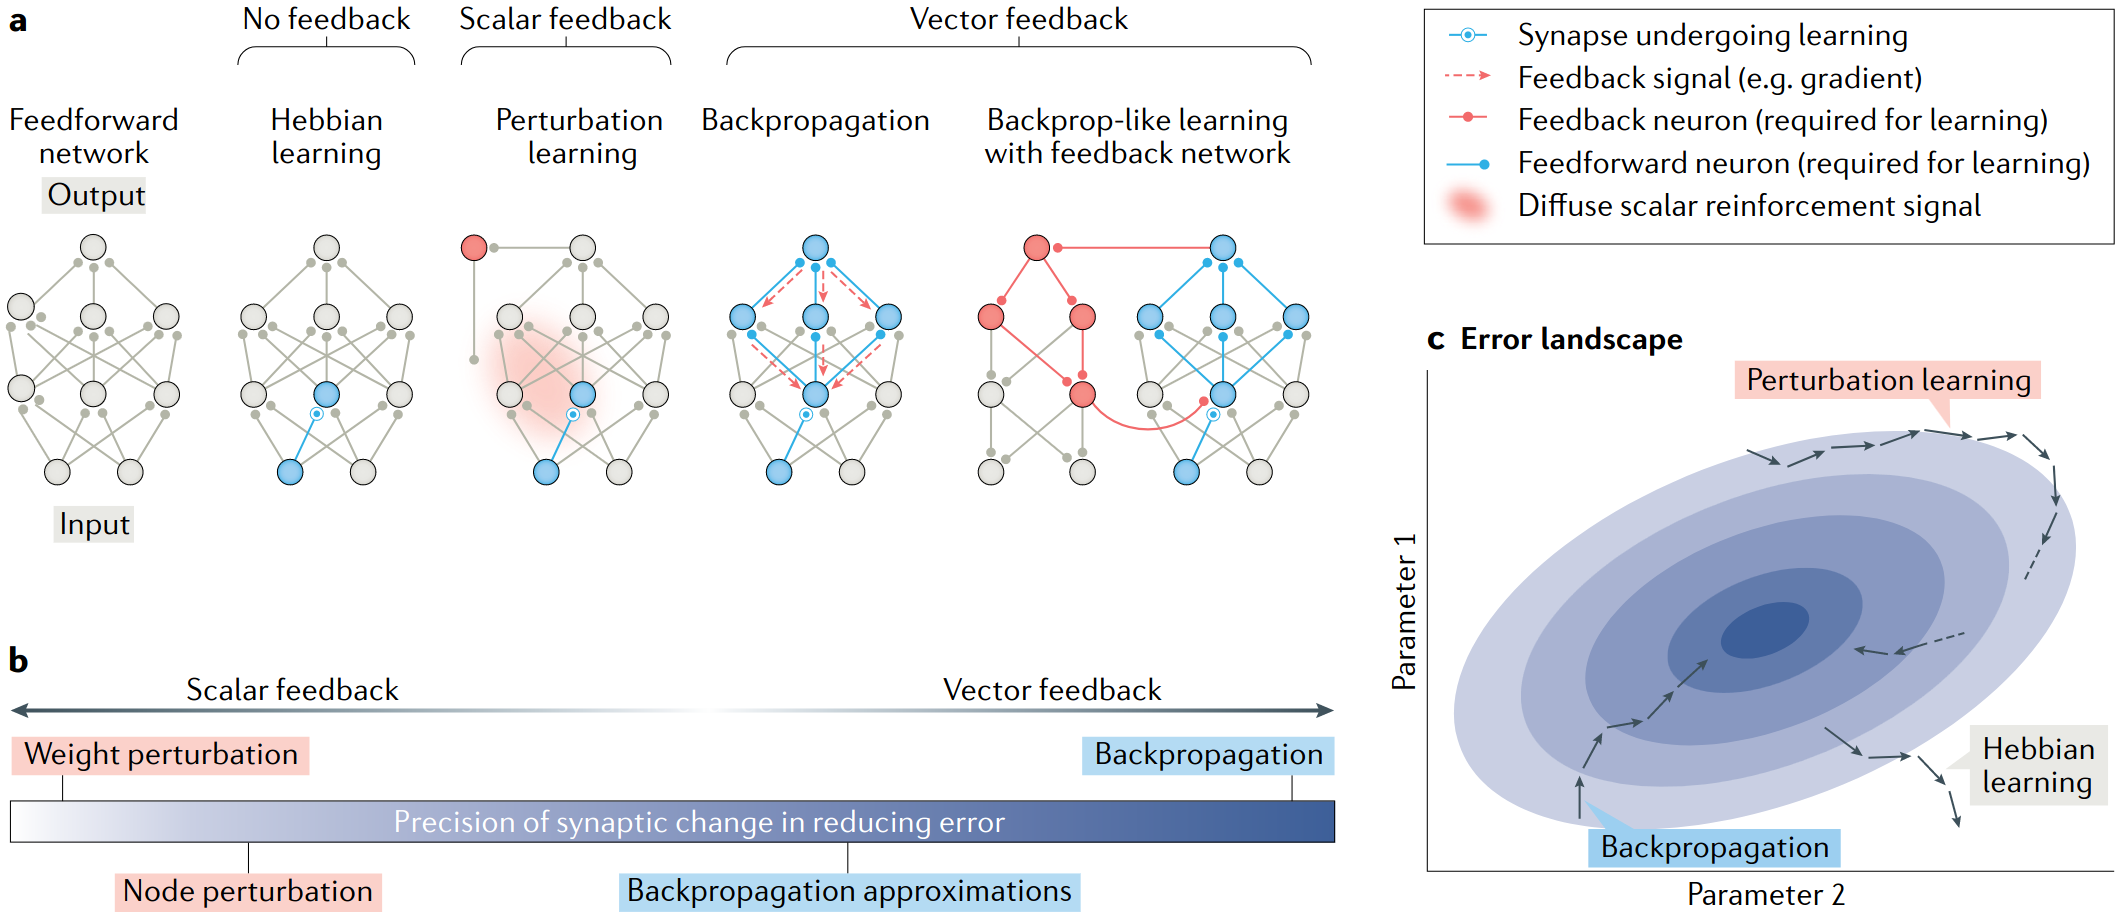
\includegraphics[width=\columnwidth]{../report/images/grad_landscape.png}
\end{frame}

%------------------------------------------------


\begin{frame}
  \frametitle{Extremum Seeking Control}
  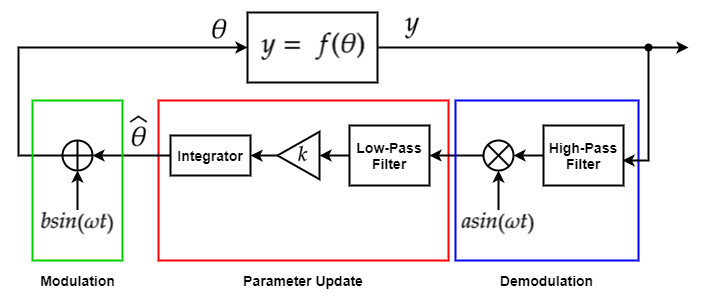
\includegraphics[width=\columnwidth]{../report/images/esc_static_optimization.png}
\end{frame}


%------------------------------------------------

\begin{frame}
  \frametitle{Extremum Seeking Control}
  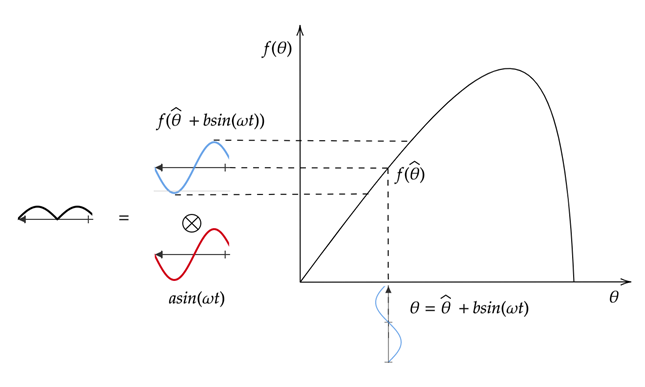
\includegraphics[width=\columnwidth]{../report/images/esc_increasing_objective.png}
\end{frame}


%------------------------------------------------


\begin{frame}
  \frametitle{Extremum Seeking Gradient}
  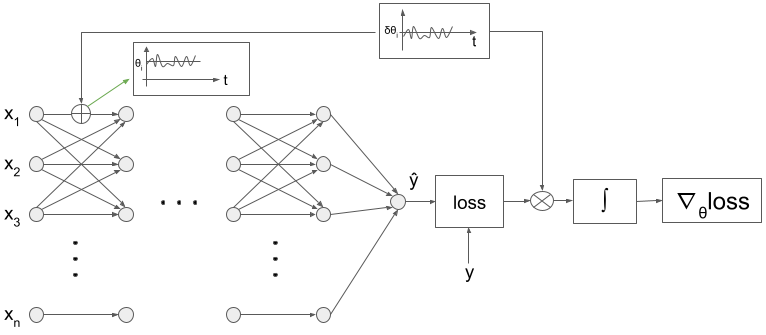
\includegraphics[width=\columnwidth]{../report/images/ESG-scheme.png}
\end{frame}


%------------------------------------------------


\begin{frame}
        \frametitle{Math proof}
\end{frame}

%------------------------------------------------

\begin{frame}
        \frametitle{Algorithm (Digital)}
\end{frame}

% ------------------------------------------------

\begin{frame}
        \frametitle{Experiments}
\end{frame}

%------------------------------------------------

\begin{frame}
        \frametitle{MeZo}
\end{frame}

%------------------------------------------------

\begin{frame}
	\frametitle{Multiple Columns}
	\framesubtitle{Subtitle} % Optional subtitle
	
	\begin{columns}[c] % The "c" option specifies centered vertical alignment while the "t" option is used for top vertical alignment
		\begin{column}{0.45\textwidth} % Left column width
			\textbf{Heading}
			\begin{enumerate}
				\item Statement
				\item Explanation
				\item Example
			\end{enumerate}
		\end{column}
		\begin{column}{0.5\textwidth} % Right column width
			Lorem ipsum dolor sit amet, consectetur adipiscing elit. Integer lectus nisl, ultricies in feugiat rutrum, porttitor sit amet augue. Aliquam ut tortor mauris. Sed volutpat ante purus, quis accumsan dolor.
		\end{column}
	\end{columns}
\end{frame}

%------------------------------------------------

\begin{frame}
	\frametitle{Definitions \& Examples}
	
	\begin{definition}
		A \alert{prime number} is a number that has exactly two divisors.
	\end{definition}
	
	\smallskip % Vertical whitespace
	
	\begin{example}
		\begin{itemize}
			\item 2 is prime (two divisors: 1 and 2).
			\item 3 is prime (two divisors: 1 and 3).
			\item 4 is not prime (\alert{three} divisors: 1, 2, and 4).
		\end{itemize}
	\end{example}
	
	\smallskip % Vertical whitespace
	
	You can also use the \texttt{theorem}, \texttt{lemma}, \texttt{proof} and \texttt{corollary} environments.
\end{frame}

%------------------------------------------------

\begin{frame}
	\frametitle{Theorem, Corollary \& Proof}
	
	\begin{theorem}[Mass--energy equivalence]
		$E = mc^2$
	\end{theorem}
	
	\begin{corollary}
		$x + y = y + x$
	\end{corollary}
	
	\begin{proof}
		$\omega + \phi = \epsilon$
	\end{proof}
\end{frame}

%------------------------------------------------

\begin{frame}
	\frametitle{Equation}

	\begin{equation}
		\cos^3 \theta =\frac{1}{4}\cos\theta+\frac{3}{4}\cos 3\theta
	\end{equation}
\end{frame}

%------------------------------------------------

\begin{frame}[fragile] % Need to use the fragile option when verbatim is used in the slide
	\frametitle{Verbatim}
	
	\begin{example}[Theorem Slide Code]
		\begin{verbatim}
			\begin{frame}
				\frametitle{Theorem}
				\begin{theorem}[Mass--energy equivalence]
					$E = mc^2$
				\end{theorem}
		\end{frame}\end{verbatim} % Must be on the same line
	\end{example}
\end{frame}

%------------------------------------------------

\begin{frame}
	Slide without title.
\end{frame}

%------------------------------------------------

%----------------------------------------------------------------------------------------
%	CLOSING SLIDE
%----------------------------------------------------------------------------------------

\begin{frame}[plain] % The optional argument 'plain' hides the headline and footline
	\begin{center}
		{\Huge The End}
		
		\bigskip\bigskip % Vertical whitespace
		
		{\LARGE Questions? Comments?}
	\end{center}
\end{frame}

%----------------------------------------------------------------------------------------

\end{document} 